\documentclass[a4paper, 12pt]{scrartcl}

\usepackage[english]{babel}
\usepackage[utf8]{inputenc}
\usepackage{amsmath}
\usepackage{geometry}
\usepackage{caption}
\usepackage{graphicx}
\usepackage[colorinlistoftodos]{todonotes}
\usepackage{hyperref}
\usepackage{booktabs}
\usepackage{cleveref}
\usepackage{listings}
\usepackage{listings-golang}
\usepackage{makecell}
\usepackage{sectsty}
\usepackage{comment}
\usepackage{multicol}

\let\bold\textbf
\setlength\parindent{0pt}
% \todo[inline]{Add diagram here}

\title{\vspace{10mm}CS628 Assignment 1 \\ $2018\text{-}19$  II Semester \\ \vspace{1cm} \textbf{Design Report for Secure Key-Value File Sharing}}
\subtitle{\vspace{4mm}\includegraphics[width=\textwidth, height=10cm]{images/cs628.png}\vspace{20mm}}
\author{Aniket Pandey $(160113)$ \hspace{5mm} $\cdot$ \hspace{5mm} Ashish Kumar $(160160)$ \\ \textit{B.S MTH} \hspace{45mm} \textit{B.Tech CSE}}
\date{\today}

\geometry{
a4paper,
total={180mm,260mm},
left=15mm,
top=15mm,}

%\sectionfont{\fontsize{15}{15}\selectfont}
%
%\title{%
%   \includegraphics[width=13cm, height=5cm]{cs628.png}
%}

\begin{document}
\clearpage\maketitle
\thispagestyle{empty}
\newpage

%\begin{center}
%	\includegraphics[width=13cm, height=5cm]{cs628.png}
%\end{center}

\section{A simple, but secure client}
\textbf{Purpose:} To maintain \textbf{Confidentiality} and \textbf{Integrity} of data without any regards to Availability.
\textbf{Note:} \textit{KeyAddr} field in every struct to protect against \textbf{key-value-swap} attack.

\begin{multicols}{2}

\begin{center}
	\textbf{USER Structure}
\end{center}

\begin{center}
	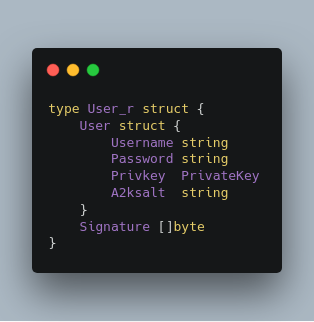
\includegraphics[width=7cm, height=6cm]{images/user.png}
\end{center}

\columnbreak

\begin{center}
	\textbf{INODE Structure}
\end{center}

\begin{center}
	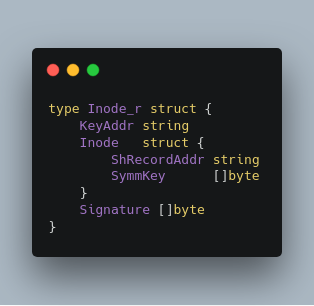
\includegraphics[width=7cm, height=6cm]{images/inode.png}
\end{center}

\end{multicols}

\subsection{InitUser (username string, password string)}
\begin{enumerate}
	\itemsep0em

    \item Obtain $UserAddr = Argon2Key("<password>+<username>", "<username>", 16)$. This will generate a 32 character address. This is where the User data will be stored.
    \item Generate a new $key = Argon2Key("<username>+<password>", "<username>", 16)$ for symmetric encryption and HMAC Signature. Sign \textit{User\_r.User} with HMAC scheme, store the signature in \textit{User\_r.Signature}. Encrypt the \textit{User\_r} struct data with AES-Cipher Feedback Mode using the same key.
	\item Generate an RSA Key-pair. Push the public key to the Public Key Server. Store the Private Key along with other fields in User\_r struct. Generate a random 16 byte symmetric key and store in user struct. This key will be used in the future to sign and encrypt inode structures.
	\item Call $DatastoreSet(key, ciphertext)$ to publish the encrypted User information in Data Server.
\end{enumerate}

\subsection{GetUser (username string, password string)}
\begin{enumerate}
	\itemsep0em

	\item Get the "key" and "address" with Argon2Key invocation. Errors suggest either incorrect username or password. Calculate the key for CFBDecrypter(), and obtain the decrypted \textit{User\_r} structure.
	\item Check HMAC hashes of $User\_r.User$ and $User\_r.Signature$ for any tampering. If all checks are satisfied, return the $User\_r.User$ structure.
\end{enumerate}

\subsection{(User) StoreFile (filename string, data []byte)}
\begin{enumerate}
	\itemsep0em
	\item Obtain $InodeAddr = SHA256 ( SHA256(<username>+<password>+<filename>) )$. This is where the Inode structure for "Username"-"Filename" will be stored (Refer to the figure).
	\item Generate a random address (key) and AES-CFB key for storing and encrypting \textit{SharingRecord\_r} structure respectively. Fill the Inode structure. Sign it using Author's Symmetric key and store HMAC signature in $Inode\_r.Signature$. Encrypt $Inode\_r$ with Author's Symmetric key. Call \textit{DataStoreSet(InodeAddr, encrypted Inode\_r)}.
	\item Check if a $SharingRecord\_r$ structure exists. If so, delete all the existing data blocks and write the new data in iterations. Else, initialize a new $SharingRecord\_r$ object.
	\item Again generate a random address (key) and AES-CFB key for storing and encrypting the $Data\_r$ structure. Store these in the relevant fields of SharingRecord structure. Sign with a predecided HMAC key and store in $SharingRecord\_r.Signature$ field. Encrypt the Structure with the key decided at $Inode\_r$ and push to Data Server.
	\item Store the "data" at the "key" generated above, Encrypt it with CFBEncrypter() method. Sign it and store the data at the "key". Push to Data Server and return. 
\end{enumerate}

\begin{multicols}{2}

\begin{center}
	\textbf{SharingRecord Structure}
\end{center}

\begin{center}
	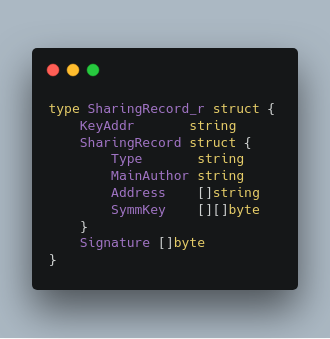
\includegraphics[width=7cm, height=6cm]{images/sharing.png}
\end{center}

\columnbreak

\begin{center}
	\textbf{DATA Structure}
\end{center}

\begin{center}
	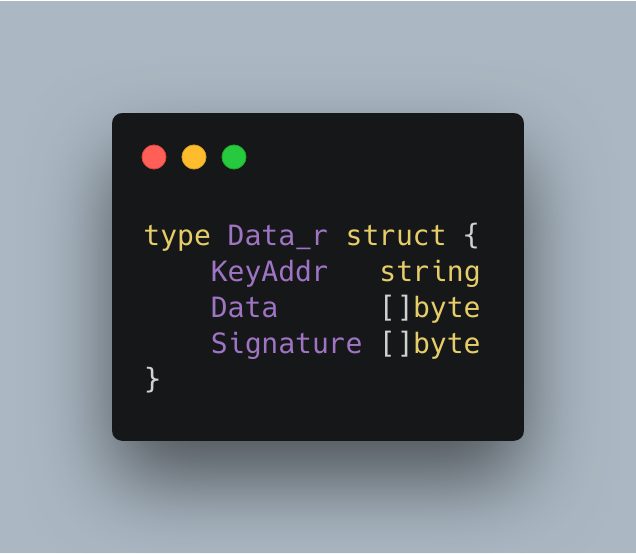
\includegraphics[width=7cm, height=6cm]{images/data.png}
\end{center}

\end{multicols}

\subsection{(User) LoadFile (filename string)}
\begin{enumerate}
	\itemsep0em
	\item Follow the method given in StoreFile() to reach, decrypt and verify the signature of the $SharingRecord\_r$ structure corresponding to "filename".
	\item Loop over the list of addresses of data chunks (via indirect pointers), decrypt and verify the HMAC signatures of each, reconstruct the entire data as a single byte array and return it.

\end{enumerate}

\subsection{(User) AppendFile (filename string, data []byte)}
\begin{enumerate}
	\itemsep0em
	\item Follow the method given in LoadFile() to reach, decrypt and verify the signature of the $SharingRecord\_r$ structure corresponding to "filename". 
	\item Create a new $Data\_r$ block and append its generated address to the list of addresses in SharingRecord structure. Push the block to DataStore and return.
	\item \textbf{NOTE:} We are not verifying the integrity of previous data blocks during AppendFile(), considering the unnecessary overhead of re-encryptions/decryptions.
\end{enumerate}

\section{Sharing and revocation}

\subsection{(User) ShareFile (filename string, recipient string)}
\begin{enumerate}
	\itemsep0em
	\item Get Inode and verify its integrity. Pass the SharingRecord Address and key to receiver. 
	\item $collected\_info = Inode\_r.Inode.(Symmkey + ShRecordAddr)$. Recieve the Public key of receiver from the Public Key Server.
	\item $sharing = PubKey_{recipient}(encrypt(collected\_info)) + PrivKey_{user}(sign(collected\_info))$, to maintain confidentiality and integrity in case of a \textbf{Man in the Middle attack} while sharing the message offline. 
\end{enumerate}

\subsection{(User) ReceiveFile (filename string, sender string, msgid string)}
\begin{enumerate}
	\itemsep0em
	\item Decrypt "msgid" using Private Key of User, verify the integrity using Public Key of Sender. Obtain the Address and "key" for CFB-Decryption of SharingRecord structure of the concerned data(value) and proceed ahead.
	\item Create an Inode for the receiver user using Argon2Key, with the method described in StoreFile(). Store the info in the Inode, store the RSA signature and encrypt $Inode\_r$ structure with Public key of User. Return.
\end{enumerate}

\subsection{(User) RevokeFile (filename string)}
\begin{enumerate}
	\itemsep0em
	\item Go upto the SharingRecord structure corresponding to "filename" and verify its integrity.
	\item From the Inode of User, change the encryption key and the address of $SharingRecord\_r$ structure and re-encrypt it with a new key. Similarly, change the address of the actual data ($SharingRecord\_r.Address$).
	\item Iterate over all data-blocks and re-encrypt them with fresh symmetric key. Also, store each of them at new addresses. Store these new key and addresses in the corresponding $SharingRecord\_r$ structure. \textbf{NOTE:} This is to prevent any further misuse by a distrusted user who knows the original key and addresses of data blocks.
\end{enumerate}

\section*{Design Changes (Post Review and Implementation)}

\begin{enumerate}
	\itemsep0em
	\item Previously, we had used RSA encryption scheme for Inode struct. However, due to length constraint and general inefficiency, we switched to AES-CFB symmetric encryption scheme.  
	\item The address where we store Inode struct was previously generated using Argon2, now we are using two consecutive invocations of SHA256, given the high time and resource requirement by Argon2.
	\item Updates in few points to enhance general readability. 
\end{enumerate}


\end{document}
